% Chapter 4

\chapter{Implementation Details} % Write in your own chapter title
\label{Chapter4}
\lhead{Chapter 4. \emph{Implementation Details}} % Write in your own chapter title to set the page header

\section{Implementation}
The system consists of five major modules i.e. Marker Hardware, Audio Hardware, Controller Application, Player Application and LMS Web Application. Implementation detail of each module is discussed below.

\section{Overall Project Structure}
This diagram shows how the modules are connected and how the effort is implemented to develop modules and connect them to form a Digital Board Marker system.

\begin{figure}[h]
  \centering
  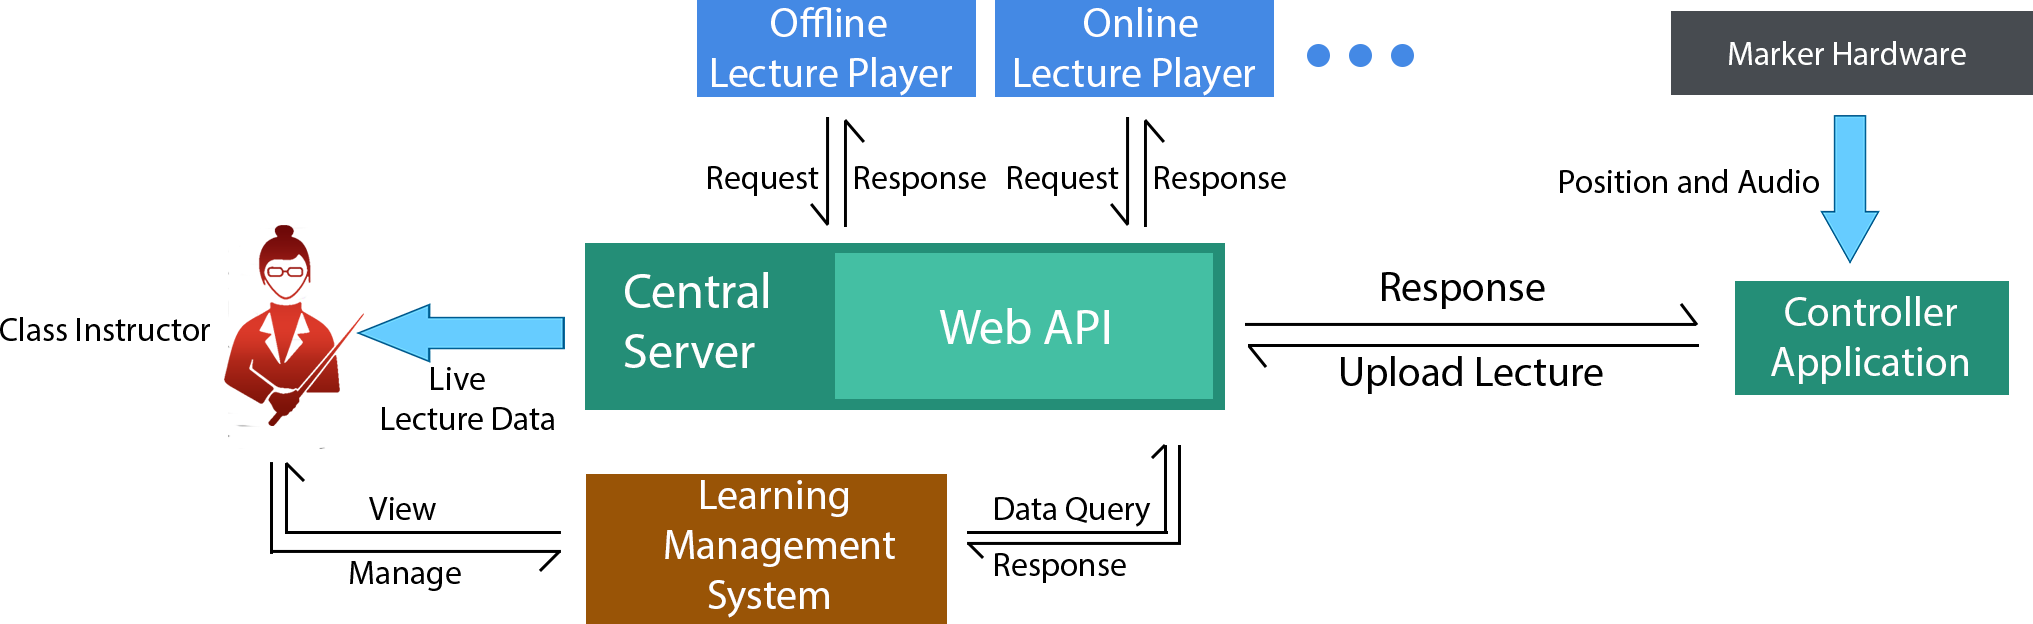
\includegraphics[width=15cm, height=7cm]{Project Structure}
  \caption{Overall Project Structure}
\end{figure}

\section{Marker Hardware}
The role of this module is to give orientation and tip pressure of the marker. The module sends data packet that contain encoded orientation of marker in 3d space in form of Euler angles.

\subsection{Requirements Addressed}


\begin{longtable}{|C{1cm}|>{\raggedright\arraybackslash}p{10cm}|C{2cm}|}

\hline


\multicolumn{1}{|>{\centering\arraybackslash}p{1cm}|}{\textbf{\#}} &
\multicolumn{1}{>{\centering\arraybackslash}p{10cm}|}{\textbf{Requirements}}
    & \multicolumn{1}{>{\centering\arraybackslash}p{2cm}|}{\textbf{Priority}}\\
\hline
% Row 1
1 &
Determine orientation of board marker and calculate respective Euler angles &
HIGH \\
\hline

2 &
Transmit the calculated Euler angles to desktop app via nrf24l01 module &
HIGH \\
\hline

3 &
Transmit the calculated Euler angles to desktop app via RS232 serial connection &
LOW \\
\hline

4 &
Turn on using 3.6 volts Li-po battery with Boost converter circuit &
MEDIUM \\
\hline

5 &
Build battery charging circuit within board marker &
LOW \\
\hline

6 &
Implement RGB Led for positioning purpose (Input for camera module) &
HIGH \\
\hline

\caption{Board Marker Hardware Requirements}

\end{longtable}

\subsection{General Flow}
\begin{itemize}

\item Board Marker try to establish wireless connection with the receiver. RGB Led fades meanwhile.
\item RGB Led turns to constant red after successful connection.
\item Accelerometer unit in the Board Marker determines the orientation data.
\item NRF24l01 wireless module in the Board Marker transmits the orientation data to Receiver wirelessly.
\item Receiver Transfers orientation data to desktop app via serial connection.

\end{itemize}

\subsection{Detailed Design}
Marker hardware has two major sub-modules named as \textbf{Transmitter} (marker itself) and \textbf{Receiver}. Below is the detail of components:
\subsubsection{Tact Tactile Switch}
Toggle switch that turns on/off the system when runs on Battery. It does not have any effect when system is running via USB cable.

\begin{figure}[h]
  \centering
  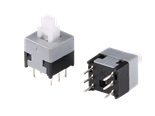
\includegraphics[width=7cm, height=7cm]{Tact Tactile Switch}
  \caption{Tact Tactile Switch}
\end{figure}

\subsubsection{USB DC-DC Boost Converter}
Converts the 3.7V to 5V to turn on and constantly run the Arduino nano prototype board. This sub-module has built-in charging circuit that charges the battery through USB connection.

\begin{figure}[h]
  \centering
  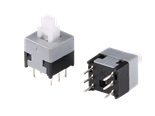
\includegraphics[width=7cm, height=7cm]{DC-DC Boost Converter}
  \caption{DC-DC Boost Converter}
\end{figure}


\subsubsection{Glowing Ball}
Round shaped glowing ball can glow in any combination of RGB colors. It is not for just looks but acts as an input to Stereo cameras for position tracking.

\begin{figure}[h]
  \centering
  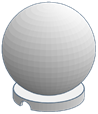
\includegraphics[width=6cm, height=7cm]{Glowing Ball}
  \caption{Glowing Ball}
\end{figure}


\subsubsection{Arduino nano}
Arduino nano acts as main processing board to which all modules and sensors are attached. It acts just like a motherboard with central processor chip soldered on mainboard.

\begin{figure}[h]
  \centering
  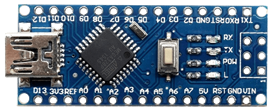
\includegraphics[width=9cm, height=6cm]{Arduino nano}
  \caption{Arduino nano}
\end{figure}


\subsubsection{Li-po battery}
600mAh 3.7V Li-po battery used to run system while there is no USB connection. Voltage may be up to 4.2 volts when fully charged. \\
\underline{DC-DC Boost Converter} is hooked up with the battery that charges the battery as well as raises its voltage to 5V to make the \underline{Board Marker Transmitter} working properly.
\newpage
\begin{figure}[h]
  \centering
  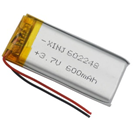
\includegraphics[width=7cm, height=6cm]{Li-po Battery}
  \caption{Li-po Battery}
\end{figure}


\subsubsection{dc-le14112 RGB Led}
3W RGB Led used to create custom color of choice, the corresponding color that is required for position sensing can glow in Glowing ball. It may be given external power source but, in our case, it is directly connected to \underline{Arduino nano}.

\begin{figure}[h]
  \centering
  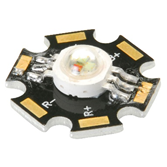
\includegraphics[width=7cm, height=7cm]{RGB Led}
  \caption{RGB Led}
\end{figure}


\subsubsection{MPU-6050}
MPU-6050 or GY-521 board contains accelerometer and gyroscope packed in a single chip. It senses the orientation of the object. It is connected to \underline{Arduino nano} via I2C bus.
\newpage
\begin{figure}[h]
  \centering
  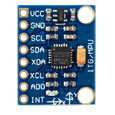
\includegraphics[width=5cm, height=6cm]{MPU-6050}
  \caption{MPU-6050}
\end{figure}


\subsubsection{nRF24L01}
nRF24L01 is a single chip radio transceiver. It is responsible for transmitting orientation data from transmitter module to receiver.

\begin{figure}[h]
  \centering
  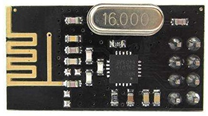
\includegraphics[width=8cm, height=4cm]{nRF24L01}
  \caption{nRF24L01}
\end{figure}

\subsection{Marker Transmitter}
The objective of the transmitter module is to extract orientation of the board marker. The challenge is the marker is changing its orientation while writing on the board. Transmitter module is designed as a back cap of board marker. It is attached to the board marker to record orientation of marker. The role of this sub-module is to transmit the tip pressure and orientation of marker in space. Further details of each part constituting the transmitter are given below.

\subsubsection{Components Used}
Detailed description of electronic components excluding discrete consumer parts, e.g. wires, is given below and described above.
\newpage
\begin{figure}[h]
  \centering
  \includegraphics[width=7cm, height=9cm]{Marker Parts}
  \caption{Board Marker with Transmitter Components}
\end{figure}

\subsubsection{Component Connection Diagram}
This diagram represents how sub-modules or components are connected in Transmitter module.
\begin{figure}[h]
  \centering
  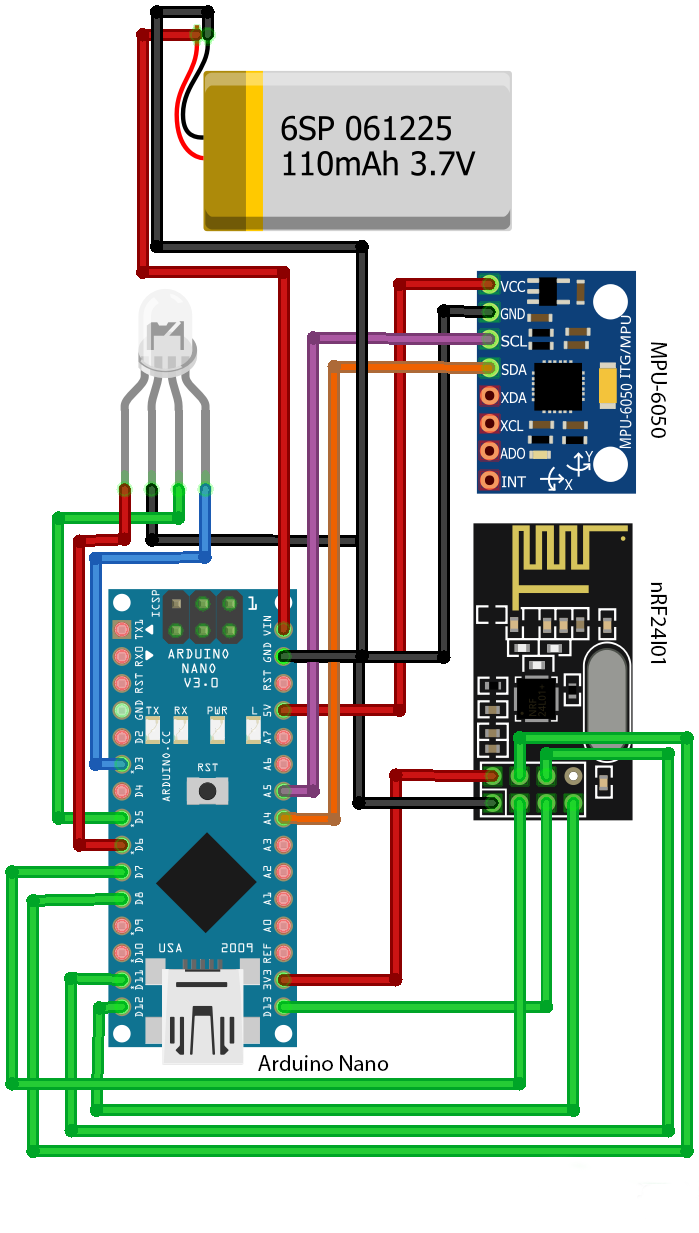
\includegraphics[width=6cm, height=9cm]{Marker Transmitter_bb}
  \caption{Component connection diagram of Board Marker Transmitter}
\end{figure}

\subsubsection{Schematic Diagram}
Schematic diagram of Board Marker Transmitter can be seen as below

\begin{figure}[h]
  \centering
  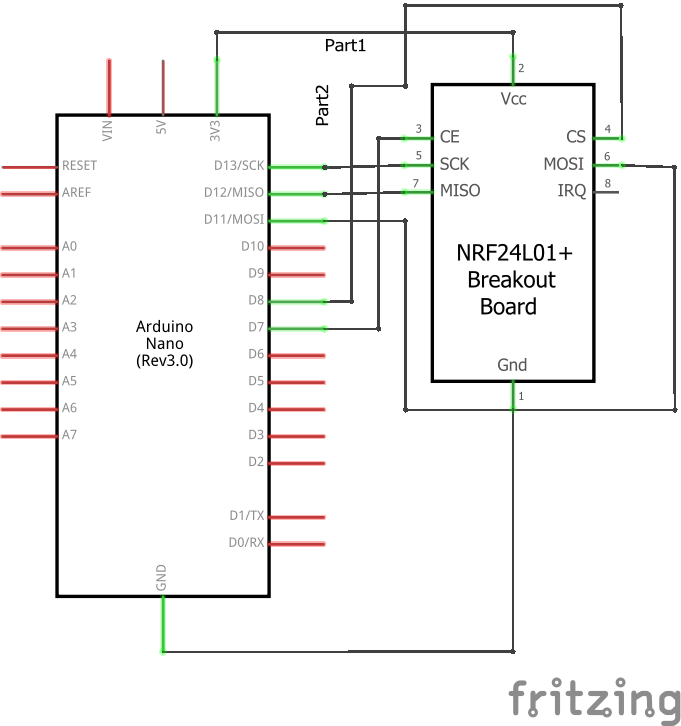
\includegraphics[width=6cm, height=8cm]{Marker Receiver_schem}
  \caption{Schematic diagram of Board Marker Transmitter}
\end{figure}


\subsubsection{General Flow}

\begin{figure}[h]
  \centering
  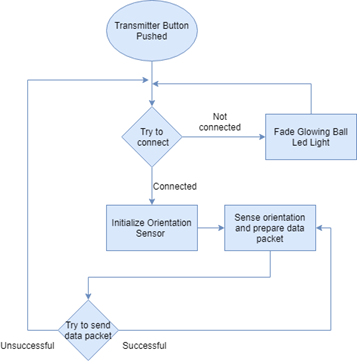
\includegraphics[width=7cm, height=10cm]{Marker Transmitter}
  \caption{General Flow of Board Marker Transmitter}
\end{figure}


\subsection{Marker Receiver}
Receiver module receives orientation data as Euler angles and transfer it to the desktop application via USB connection. As it is connected via USB so it does not need any external power source.

\subsubsection{Component Connection Diagram}

\begin{figure}[h]
  \centering
  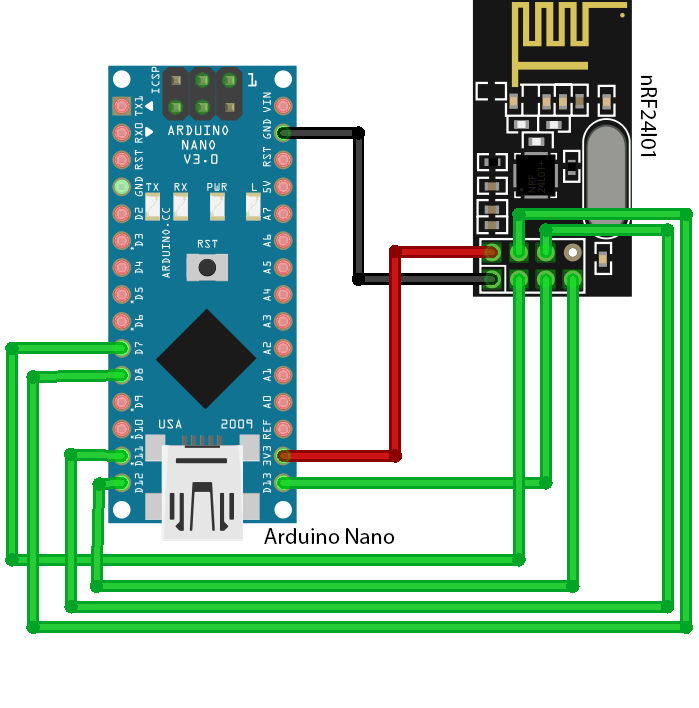
\includegraphics[width=5cm, height=7cm]{Marker Receiver_bb}
  \caption{Component connection diagram of Board Marker Receiver}
\end{figure}

\subsubsection{Schematic Diagram}
Schematic diagram that shows abstract component view of Receiver module is given below

\begin{figure}[h]
  \centering
  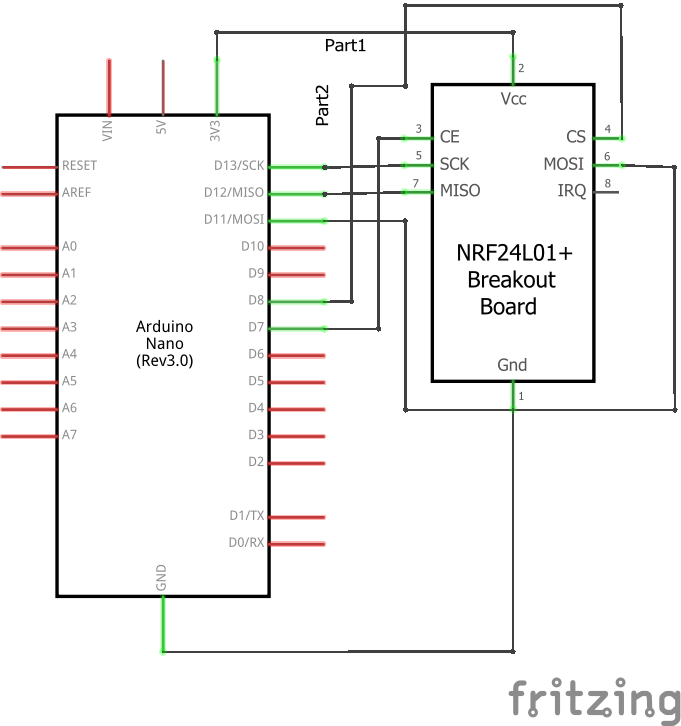
\includegraphics[width=5cm, height=7cm]{Marker Receiver_schem}
  \caption{Schematic diagram of Board Marker Receiver}
\end{figure}
\newpage
\subsubsection{General Flow}
\begin{figure}[h]
  \centering
  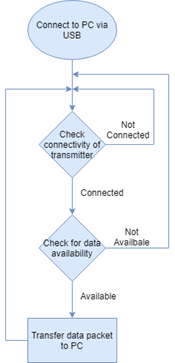
\includegraphics[width=7cm, height=9cm]{Marker Receiver}
  \caption{General Flow of Board Marker Receiver}
\end{figure}

\subsection{Rules and Assumptions}
Following are rules and cases of assumptions that are assumed to be true while normal working
\begin{itemize}

\item Board Marker Transmitter and Receiver are in range of 2 meters for less noise and preventing latency issues.
\item Pressure threshold of board marker tip is 5Pascals that is equivalent to pressure of lead pencil tip. Above this pressure, marker will write and otherwise not.
\item Glowing ball of board marker must be at least partially visible by either of the cameras. Precision of marker position decreases from Case 1 to 6. Best Accuracy in Case 1 and no output at all in Case 6.
\item User is supposed to be not touching the Marker tip while recording the lecture.
\item User is supposed to be write only in the boundary of the defined platform i.e. whiteboard. 

\end{itemize}
\newpage
\begin{figure}[h]
  \centering
  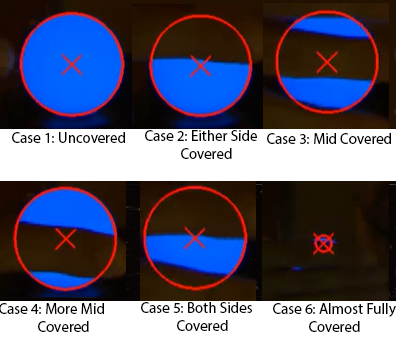
\includegraphics[width=9cm, height=8cm]{Ball cover}
  \caption{Glowing Ball Detection While Covered}
\end{figure}

\subsection{Tools and Technologies used}
List all software that are used to develop and needed to operate the developed module are detailed below.

\subsubsection{Arduino IDE v1.8.9}
Code environment in which all code for Board Maker Transmitter and Receiver is written. This IDE is numerously used as a debugging tool as well.

\subsubsection{Processing v3.5.3}
This tool is used for debugging and visualization of Board Marker Transmitter as a teapot object. In order to view Board Marker Transmitter and verify the placement of MPU-6050 orientation sensor and latency, we visualized the teapot object moving in the window of Processing software. Following parameters and properties are visualized and debugged.

\begin{itemize}

\item Correct orientation data packet format of Board Marker Transmitter.
\item Generation of noise with respect to obstacles and distance involved while data transmission.
\item Latency in data transmission with respect to obstacles and distance involved while data transmission.

\end{itemize}

Sample image of object is given below
\newpage
\begin{figure}[h]
  \centering
  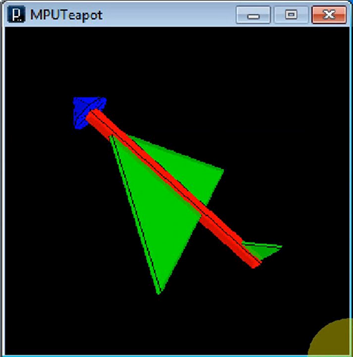
\includegraphics[width=11cm, height=10cm]{Teapot}
  \caption{Marker Orientation Image in Processing Software}
\end{figure}

\section{Audio Hardware}
Role of Audio Hardware is to establish a wireless voice communication between Teacher and Controller Application. The module wirelessly transmits the voice of Teacher to controller app. The module works on 2.4G frequency band approved and approved by RoHS.

\subsection{Requirements Addressed}
\begin{longtable}{|C{1cm}|>{\raggedright\arraybackslash}p{10cm}|C{2cm}|}

\hline


\multicolumn{1}{|>{\centering\arraybackslash}p{1cm}|}{\textbf{\#}} &
\multicolumn{1}{>{\centering\arraybackslash}p{10cm}|}{\textbf{Requirements}}
    & \multicolumn{1}{>{\centering\arraybackslash}p{2cm}|}{\textbf{Priority}}\\
\hline
% Row 1
1 &
Transfer Voice data from one point to another. &
HIGH \\
\hline

2 &
Transfer Voice data from transmitter to receiver wirelessly.  &
HIGH \\
\hline

3 &
Transmitter should be standalone in terms of power. &
HIGH \\
\hline

4 &
Receiver should output voice data as analogue audio wave. &
MEDIUM \\
\hline

5 &
Implement noise control knob in transmitter. &
MEDIUM \\
\hline


\caption{Audio Hardware Requirements}

\end{longtable}

\subsection{General Flow}

\begin{itemize}

\item Transmitter try to connect to the Receiver
\item After a successful connection, Transmitter reads analogue signal and converts it into digital PWM wave.
\item Transmitter then starts transmitting the voice data through nRF24L01 module.
\item Voice data arrives at nRF24L01 of Receiver.
\item Receiver converts the incoming signal into audio wave.


\end{itemize}

\subsection{Detailed Design}
Audio hardware has two major sub-modules named as Transmitter and Receiver

\subsubsection{Electret Microphone}
9767 Condenser Electret Microphone used to capture voice.
\begin{figure}[h]
  \centering
  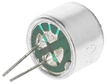
\includegraphics[width=4cm, height=4cm]{Mic}
  \caption{Electret Microphone}
\end{figure}


\subsubsection{100K Resistor}
Used to adjust input gain of microphone. It is connected with the \underline{Microphone Circuit}.

\begin{figure}[h]
  \centering
  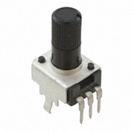
\includegraphics[width=5cm, height=4cm]{Pot}
  \caption{100K Resistor}
\end{figure}

\subsubsection{Microphone Circuit}
An electric circuit implemented on a dotted Veroboard. It transfers the voltage change due to microphone to the \underline{Arduino nano} mainboard


\subsubsection{Input Audio Socket}
3.5mm Audio Socket that is used to input the audio wave. It acts as mono input audio channel.

\subsubsection{Output Audio Socket}
3.5mm Audio Socket that is used to output the audio wave. It acts as mono output audio channel.

\begin{figure}[h]
  \centering
  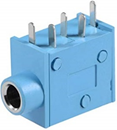
\includegraphics[width=5cm, height=6cm]{3.5mm jack}
  \caption{Audio Jack}
\end{figure}

\subsubsection{Arduino nano}
Arduino nano acts as main processing board to which all modules and sensors are attached. It acts just like a motherboard with central processor chip soldered on mainboard.

\begin{figure}[h]
  \centering
  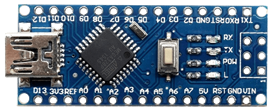
\includegraphics[width=6cm, height=4cm]{Arduino nano}
  \caption{Arduino nano}
\end{figure}

\subsubsection{nRF24L01 Adapter}
5V to 3.3V nRF24L01 adapter gives constant 3.3V from input 5V. It prevents nRF24L01 module not to drain power from \underline{Arduino nano} mainboard.


\begin{figure}[h]
  \centering
  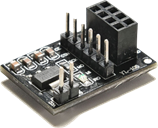
\includegraphics[width=8cm, height=6cm]{nrf Adapter}
  \caption{nRF24L01 Adapter}
\end{figure}

\subsubsection{Noise Reduction Circuit}
The circuit is used to reduce random noise with the help of gradual grounding the input audio wave.


\subsubsection{nRF24L01}
nRF24L01 is a single chip radio transceiver. It is responsible for transmitting voice data from transmitter module to receiver.

\begin{figure}[h]
  \centering
  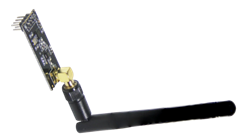
\includegraphics[width=8cm, height=6cm]{nrf Antenna Version}
  \caption{nRF24L01 Antenna Version}
\end{figure}

\subsection{Audio Transmitter}
The objective of the Audio Transmitter is to get voice data from microphone and transmit it to the Audio Receiver. After getting the data from microphone, it converts analogue audio data into a digital Pulse Width Modulation or PWM wave.

\subsection{Components Used}
Detailed description of electronic components excluding discrete consumer parts, e.g. wires, is given below and described above.

\begin{figure}[h]
  \centering
  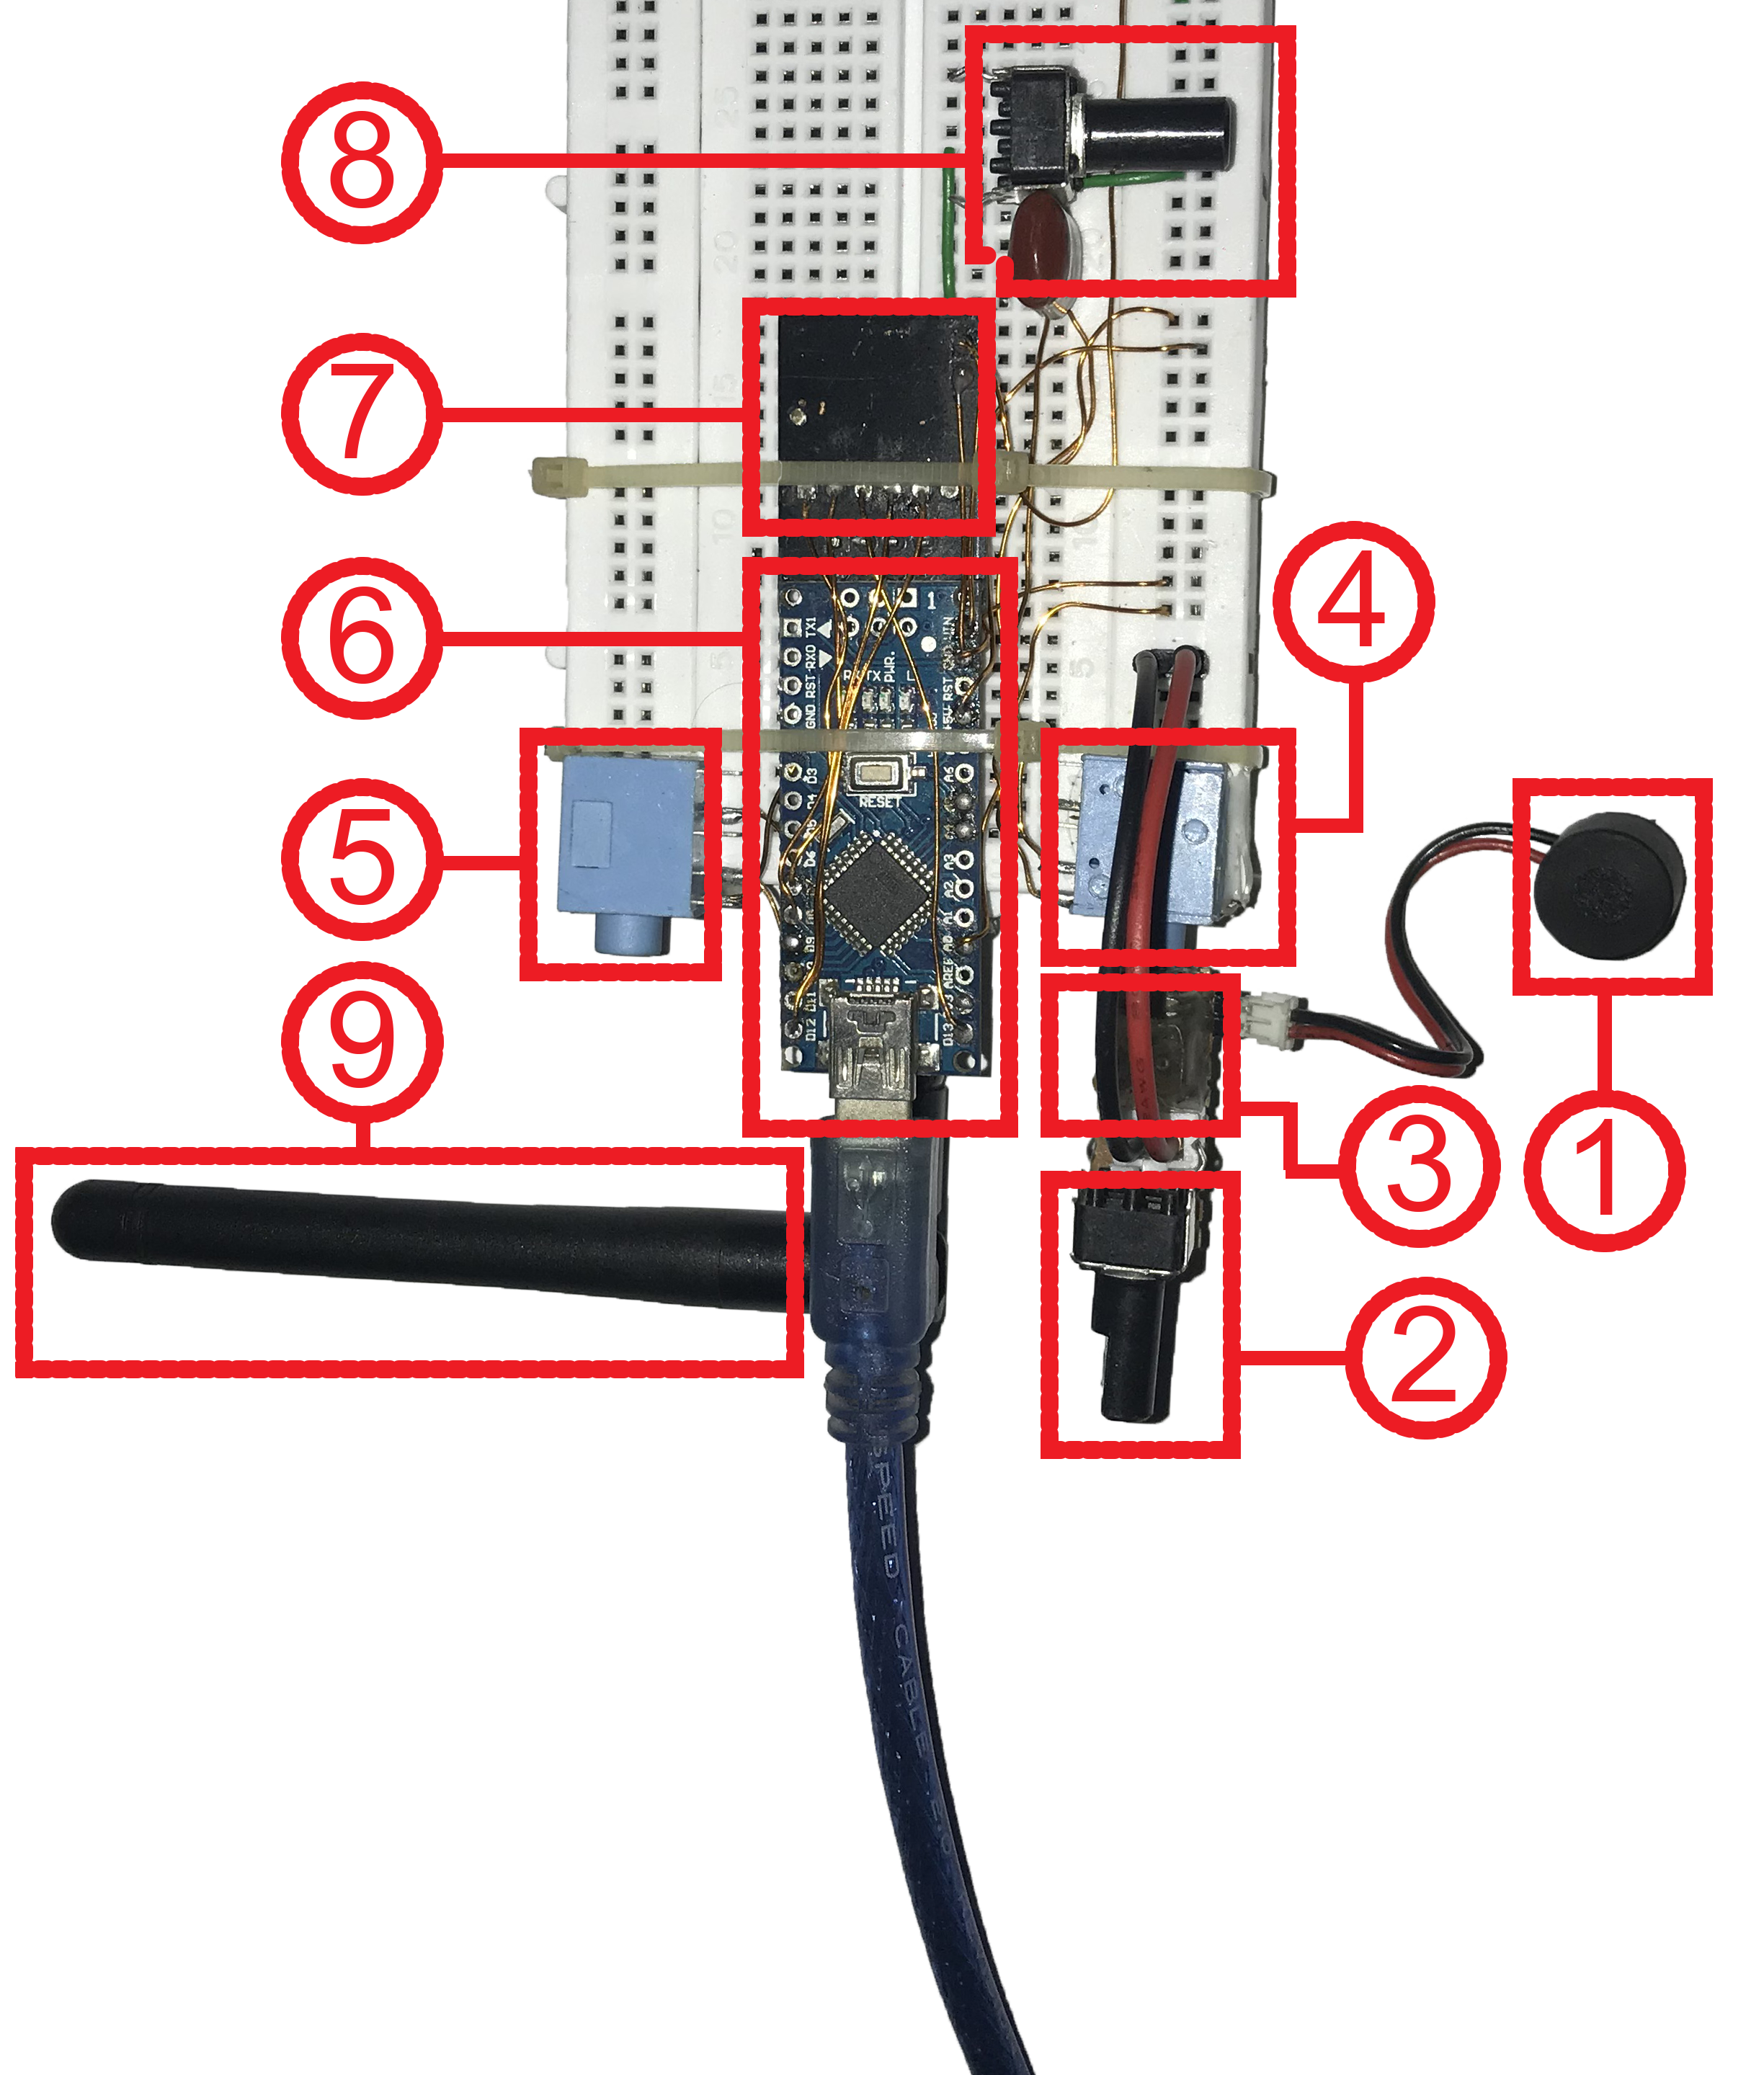
\includegraphics[width=6cm, height=8cm]{Audio Trans num}
  \caption{nRF24L01 Audio Transceiver Component Detail}
\end{figure}

\subsection{Component Connection Diagram}
This diagram represents how sub-modules or components are connected in Transceiver module.


\begin{figure}[h]
  \centering
  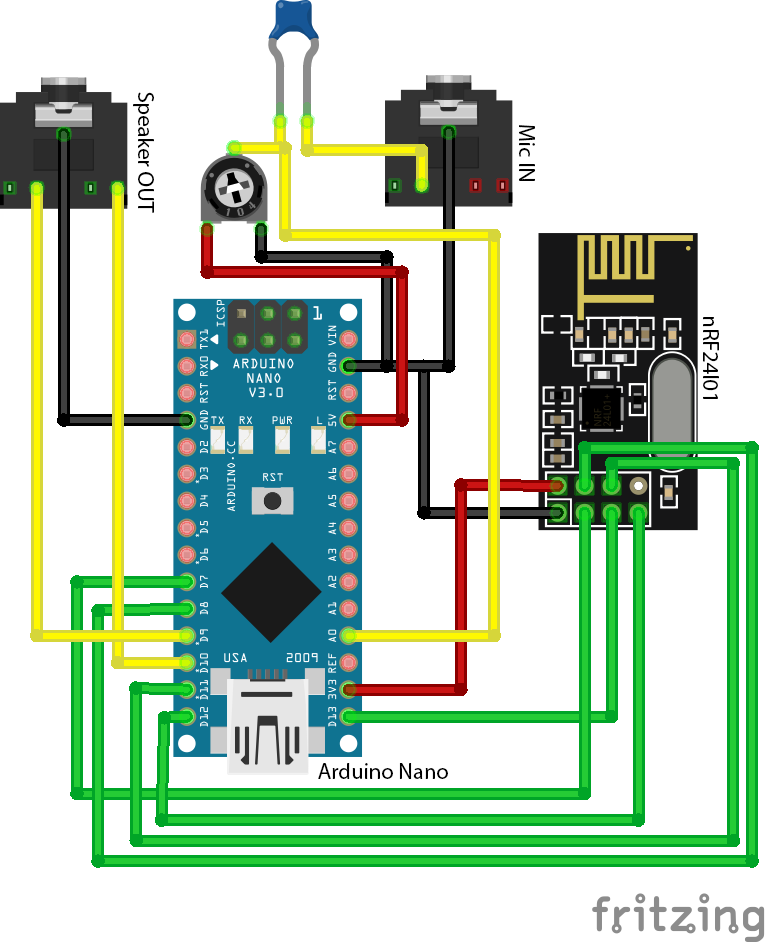
\includegraphics[width=5cm, height=7cm]{Audio Receiver_bb}
  \caption{Audio Transceiver Component Connection Diagram}
\end{figure}


\subsection{Schematic Diagram}

\begin{figure}[h]
  \centering
  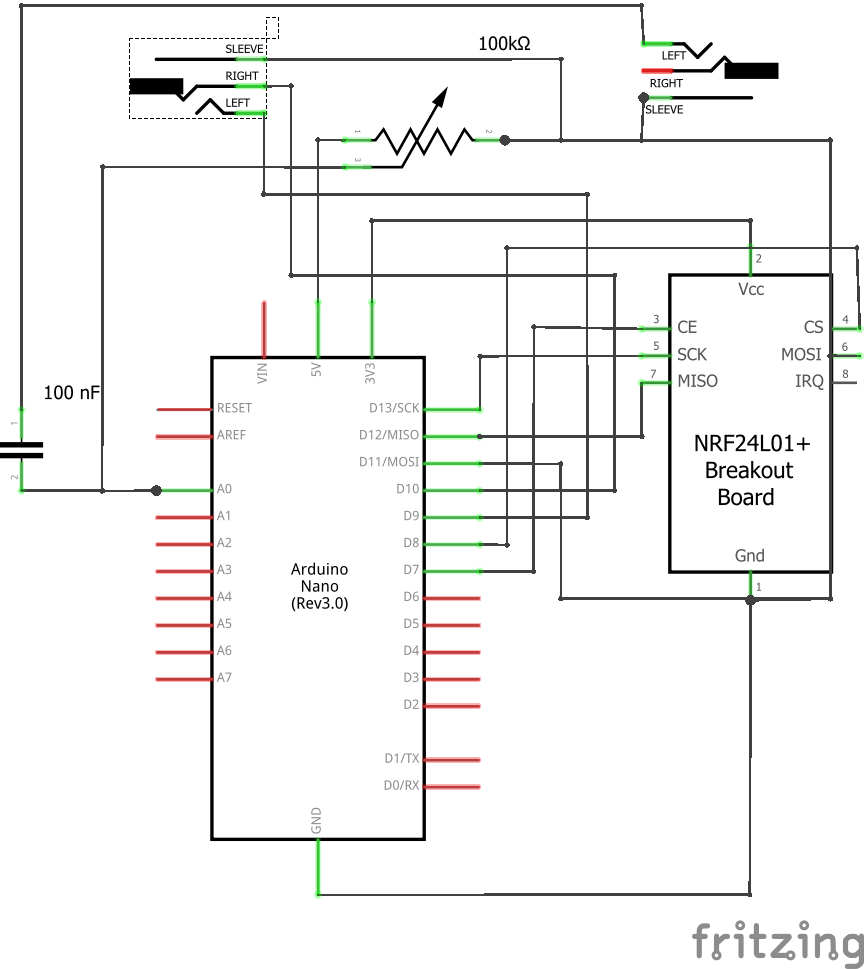
\includegraphics[width=7cm, height=8cm]{Audio Receiver_schem}
  \caption{Audio Transceiver Schematic Diagram}
\end{figure}


\subsection{General Flow}

\begin{figure}[h]
  \centering
  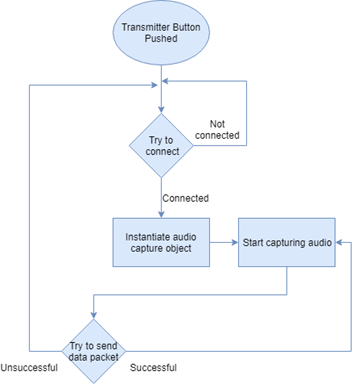
\includegraphics[width=8cm, height=9cm]{Audion transmitter flow}
  \caption{General Flow of Audio Transmitter}
\end{figure}

\subsection{Audio Receiver}
Receiver module receives audio data from transmitter. Although the Arduino nano mainboard is programmed differently but the circuit and composition of receiver module is identical to transmitter module.

\subsection{Components Used}
Detailed description of electronic components excluding discrete consumer parts, e.g. wires, is given below and described above.

\begin{figure}[h]
  \centering
  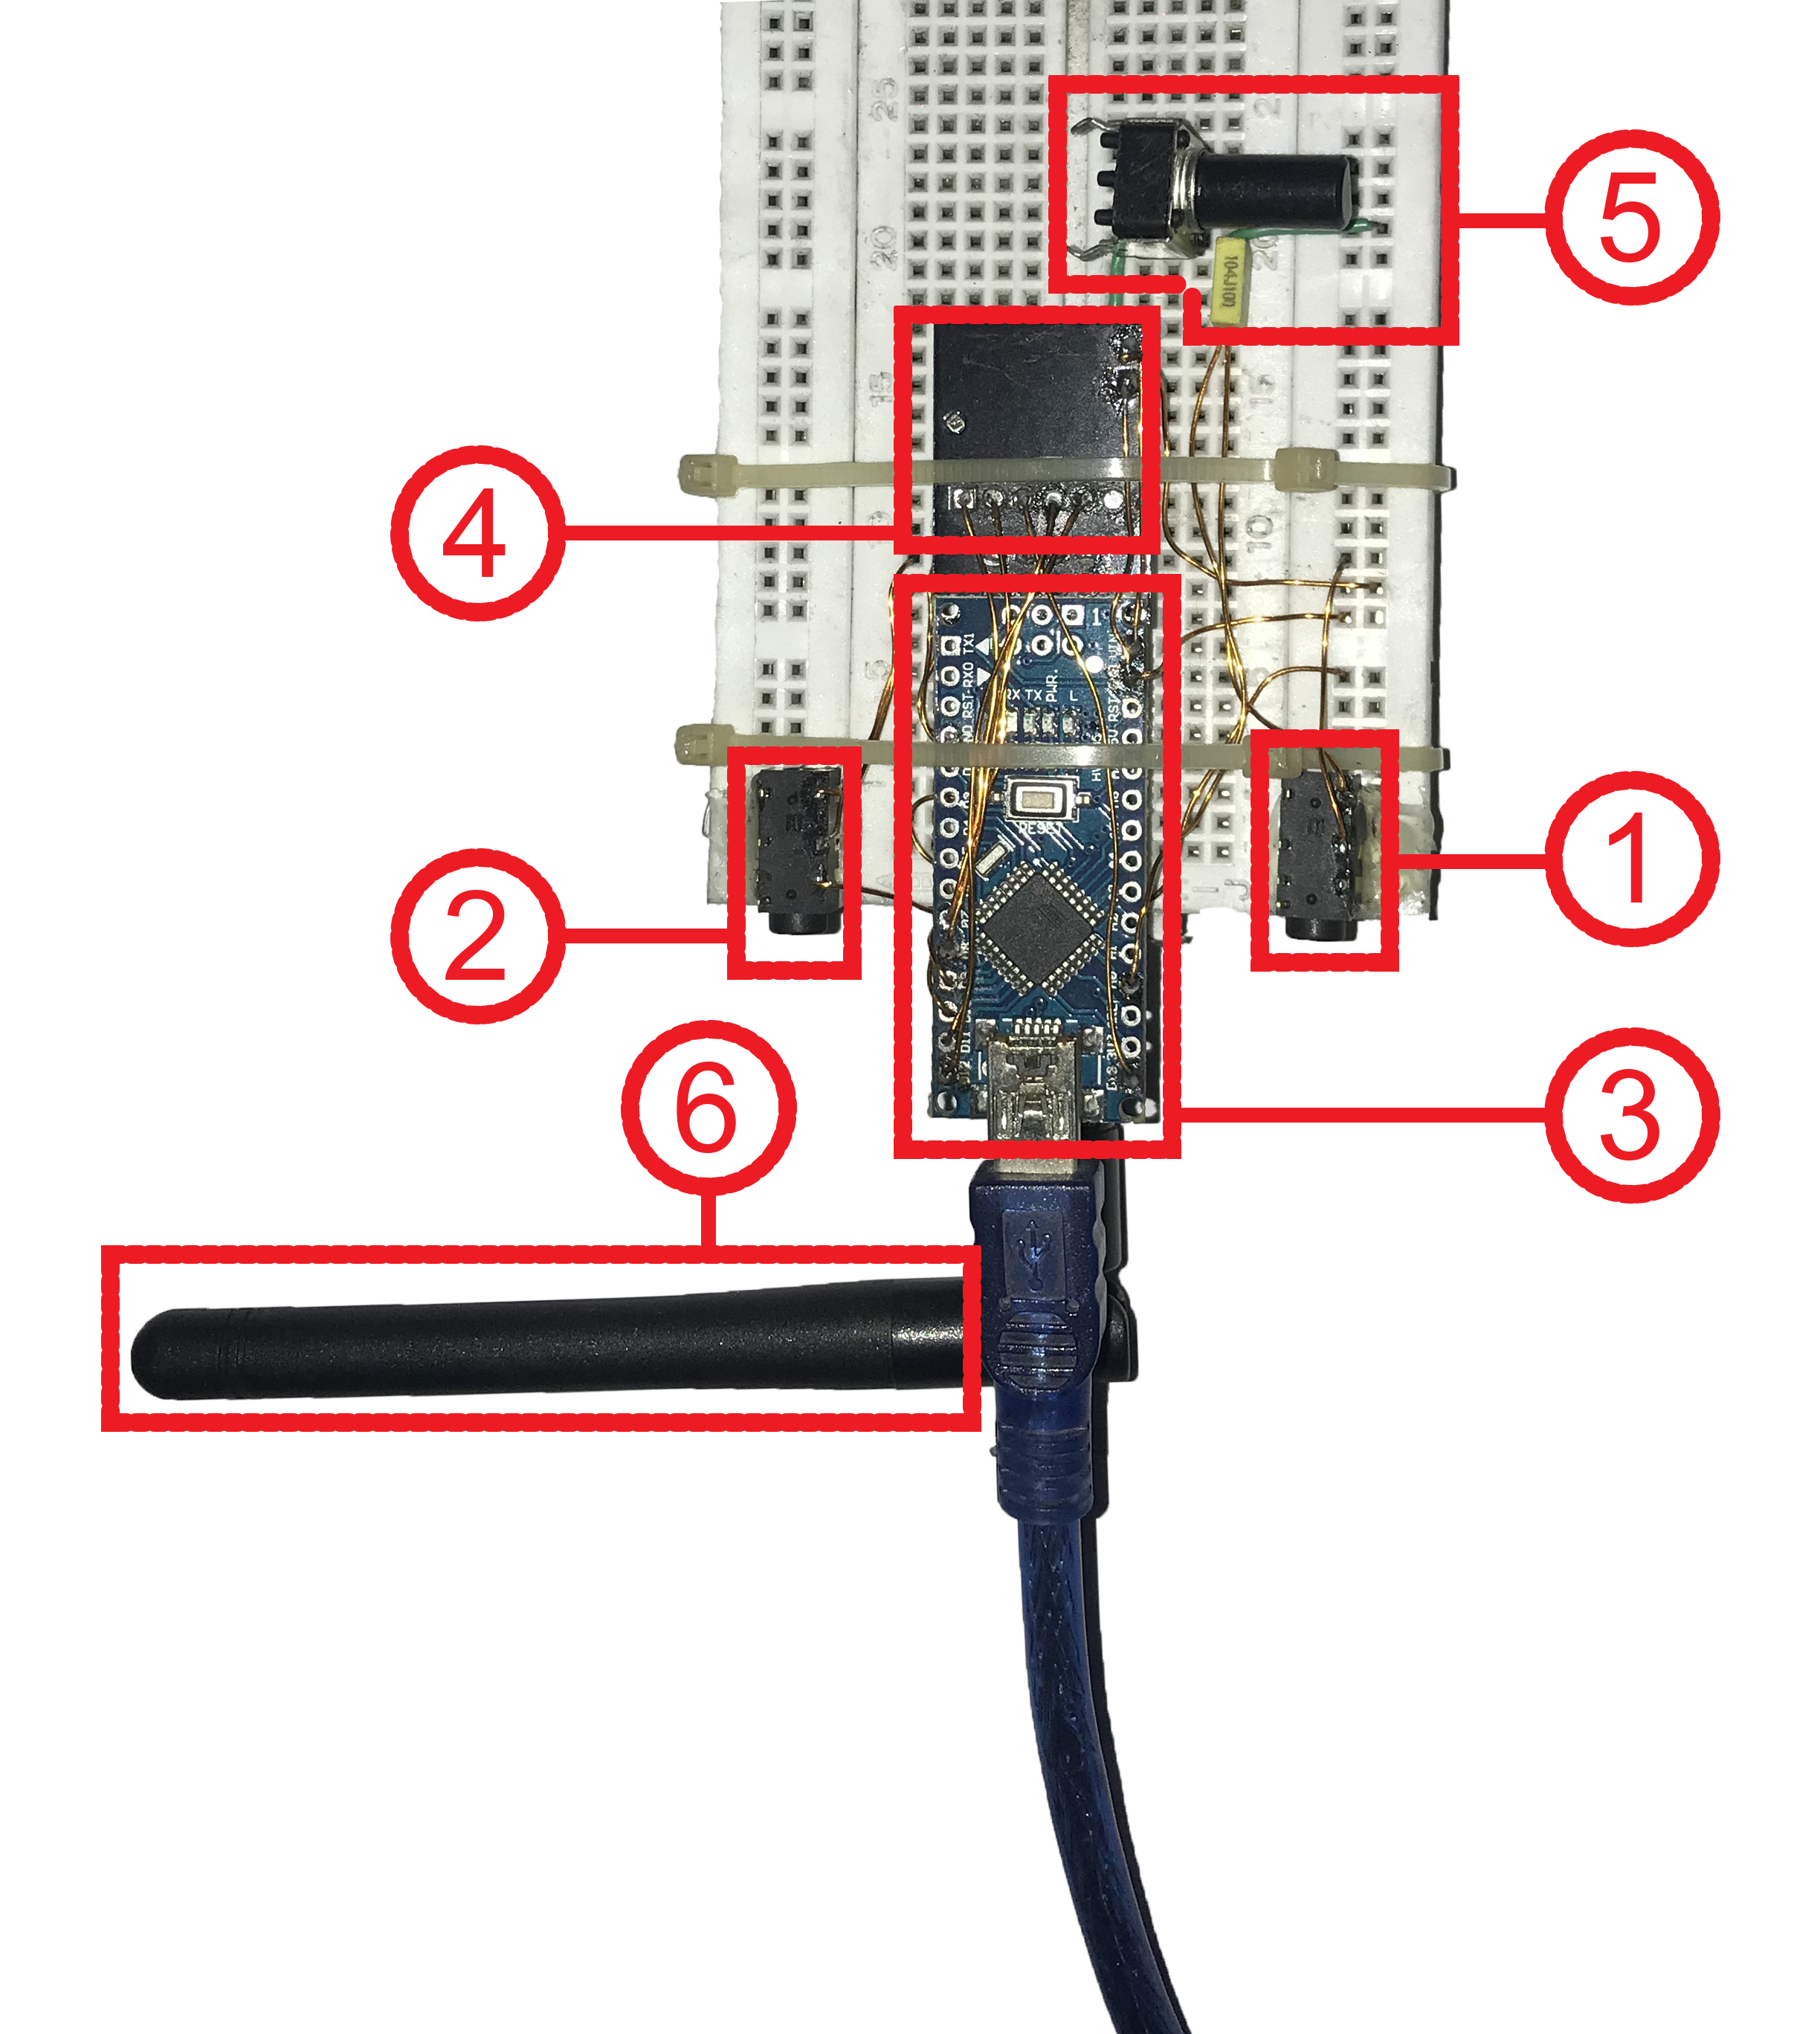
\includegraphics[width=6cm, height=7cm]{Audio Recv num}
  \caption{Component Diagram of Audio Receiver}
\end{figure}

\subsection{General Flow}

\begin{figure}[h]
  \centering
  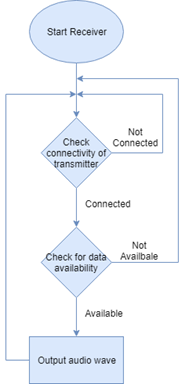
\includegraphics[width=6cm, height=7cm]{Audion Reciever flow}
  \caption{General Flow of Audio Receiver}
\end{figure}


\subsection{Rules and Assumptions}
Following are rules and cases of assumptions that are assumed to be true while normal working:

\begin{itemize}

\item Audio Transmitter and Audio Receiver must be in range of 5 meters.
\item Microphone should be in range of 10cm from the audio source i.e. speaker's mouth.

\end{itemize}

\subsection{Tools and Technologies used}
List all software that are used to develop and needed to operate the developed module are detailed below:

\subsubsection{Arduino IDE v1.8.9}
Code environment in which all code for Audio Transmitter and Audio Receiver is written. This IDE is numerously used as a debugging tool as well. 

\section{Controller Application}
This module controls the recording of lecture. It acts as a receiver end from the Marker and Audio Hardware point of view. It generates a lecture file with .dbm extension. That file is then uploaded to central server. Lecture file now can be played on the website using WebGL player or Offline player application.\\

Complete description along with UI screens of controller application are given below:

\subsection{Home Screen}
Controller application has navigation bar on left side that control panel and sub-panels that contain buttons. Buttons navigate to the corresponding form. A hierarchy that describe the categorization of forms is given below.

\begin{enumerate}

\item Home Panel
\begin{itemize}
\item Player
\item Home Screen
\end{itemize}

\item Settings Panel
\begin{enumerate}[a.]

\item Hardware Input Sub-Panel
\begin{itemize}

\item Position
\item Camera
\item Orientation
\item Filter

\end{itemize}

\end{enumerate}

\end{enumerate}

\textbf{Home Screen:} Home Screen button is clicked; home screen of Controller Application is shown. It acts just as splash indicating that application is running fine. Application show home screen by default on launch.

\begin{figure}[h]
  \centering
  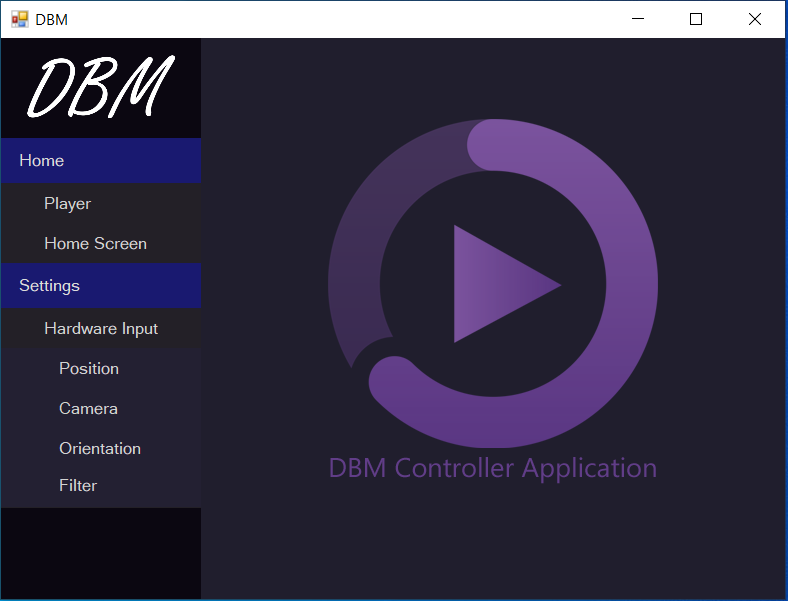
\includegraphics[width=15cm, height=15cm]{Controller App Home}
  \caption{Home Screen Controller Application}
\end{figure}

\subsection{Record Panel Screen}
When player button is clicked, application opens the lecture recording control panel. This panel contain the following controls:

\begin{enumerate}

\item Seek bar: Indicates the current playing time of the lecture video. It also indicates how much video as passed and how much is remaining.
\item Start Recording button: Lecture recording is started after pressing this button.
\item Stop Recording button: Lecture recording is stopped after pressing this button.
\item Start Playing button: Plays the recorded lecture.
\item Duster button: Press it when you want to erase a little.
\item Clear button: Press it when whole board is to be erased.
\item Enable Device Input button: Press it to enable Marker hardware and Audio hardware input to controller application for lecture recording. When disabled, mouse input is considered i.e. you will be using mouse to write on canvas.
\item Save File button: To save the recorded lecture file. It will generate a file with .dbm extension.
\item Load File button: To load the recorded lecture file. It will open a file browser from which a file with .dbm extension is selected.
\item Thickness Trackbar: Controls the line thickness of writing being written and also duster size.
\item Tick Resolution numeric up down: Controls the refresh rate of Canvas. Lower the value, higher the resolution and hence better quality but more storage required.
\item Color picker: Change the color of writing. In case you are using multiple board markers with different colors.
\item Position textbox: Indicates the current position of pointer on the Canvas. 
\item Load Saved button: Load the saved settings on local storage.
\item Save Settings button: Save the settings from local storage.
\item Canvas: Black window on which words are being written i.e. Board.

\end{enumerate}

\newpage

\begin{figure}[h]
  \centering
  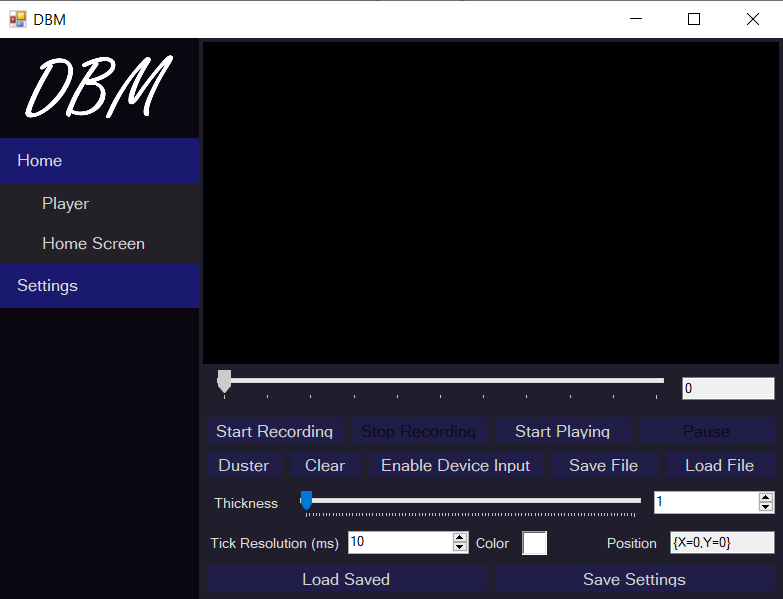
\includegraphics[width=12cm, height=11cm]{Controller Application Record Panel}
  \caption{Controller Application Record Panel}
\end{figure}

\subsection{Position Calibration Screen}
When Settings->Hardware Input->Position from navigation bar is clicked, Position Calibration form is displayed. It contains the following controls

\begin{enumerate}

\item Canvas: A container that holds visual elements of either side of board. It contains the lines of sight of each camera and red circle indicates the glowing ball position of the marker. The blue dot indicates the tip position of the marker.
\item Invert Left button: Inverts the control of left-side camera.
\item Invert Right button: Inverts the control of right-side camera.
\item Position textbox: Indicates the current tip position of the Marker Hardware.
\item Load button: Load the saved settings from local storage.
\item Save button: Save settings on local storage.

\end{enumerate}

\newpage
\begin{figure}[h]
  \centering
  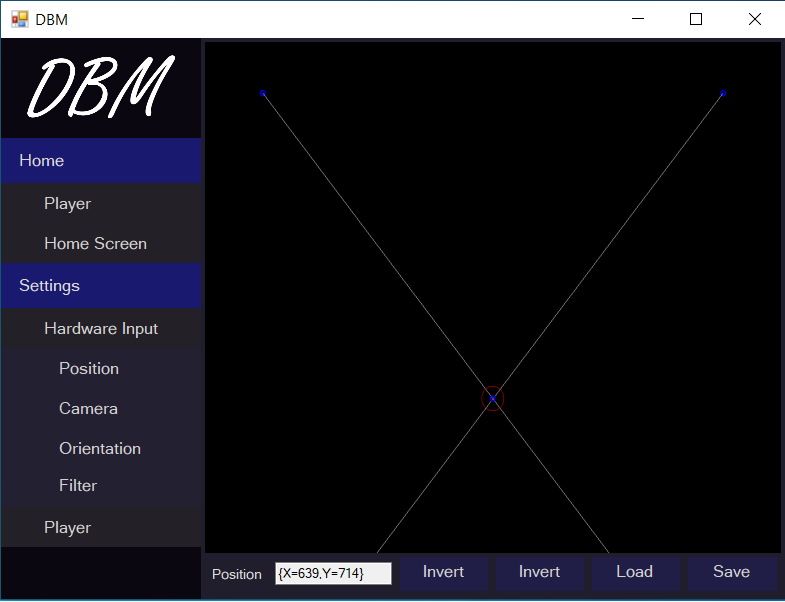
\includegraphics[width=12cm, height=11cm]{Controller App Position Calibration}
  \caption{Controller App Position Settings}
\end{figure}

\subsection{Camera Control Panel Screen}
When Settings->Hardware Input->Camera from navigation bar is clicked, Camera Control Panel form is displayed. Role of this form is to start camera stream and preview in the form window from connected cameras. It contains at least two sub-forms that contain settings of each camera. Each camera form contains the following controls:

\begin{enumerate}

\item Select Camera dropdown: Contains list of all connected cameras from which any of the cameras can be selected. Choose carefully i.e. what camera is placed on Left or Right on the board.
\item FPS textbox: The framerate of camera. Higher the framerate, better the performance. Framerate should not exceed from the mentioned framerate on camera.
\item Capture button: Start the camera capture.
\item Preview button: Camera preview is displayed on the preview box below.
\item Load Saved button: Load saved settings from the local storage.
\item Save Settings button: Save the settings on local storage.

\end{enumerate}


\begin{figure}[h]
  \centering
  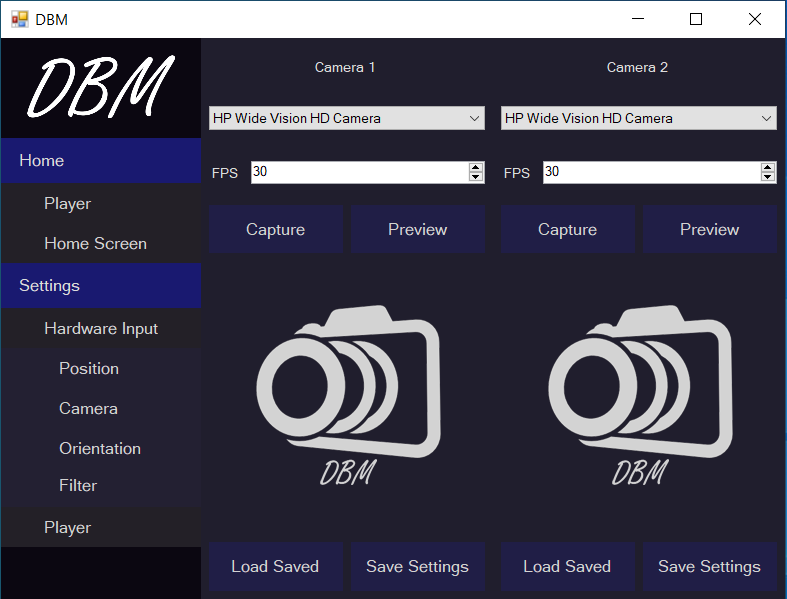
\includegraphics[width=12cm, height=11cm]{Controller App Camera Settings}
  \caption{Controller App Camera Settings}
\end{figure}

\subsection{Orientation Calibration Screen}
When Settings->Hardware Input->Orientation from navigation bar is clicked, Orientation Control Panel form is displayed. Role of this form is to calibrate and visualize the orientation of the board marker. It contains the following controls:

\begin{enumerate}

\item Start button: Starts the orientation input from Marker Hardware.
Refresh button: Refreshes the list of available communication serial ports.
\item Serial Port dropdown: Dropdown list of available serial ports. \item Choose the one with which Marker Hardware is connected.
\item Current Orientation group-box: Shows X-axis, Y-axis and Z-axis rotation of Marker Hardware along its pivot point.
\item Current Pressure textbox: Shows the amount of pressure applied on the tip of Marker.
\item Tip Offset textbox: Shows the calculated tip offset from the origin point as compared to when Marker was kept at 90 degree with the Board.
\item Apply Offset group-box: Trackbars that give offset to calculated angles alone X-axis, Y-axis and Z-axis respectively to calibrate the orientation.
\item Load Saved button: Load saved settings from the local storage.
\item Save Settings button: Save the settings on local storage.
\item Show 3d Orientation button: Opens another form that show orientation of Marker in 3d space.
\item Show 2d Orientation button: Opens another form that show orientation of Marker in 2d plane.

\end{enumerate}

\begin{figure}[h]
  \centering
  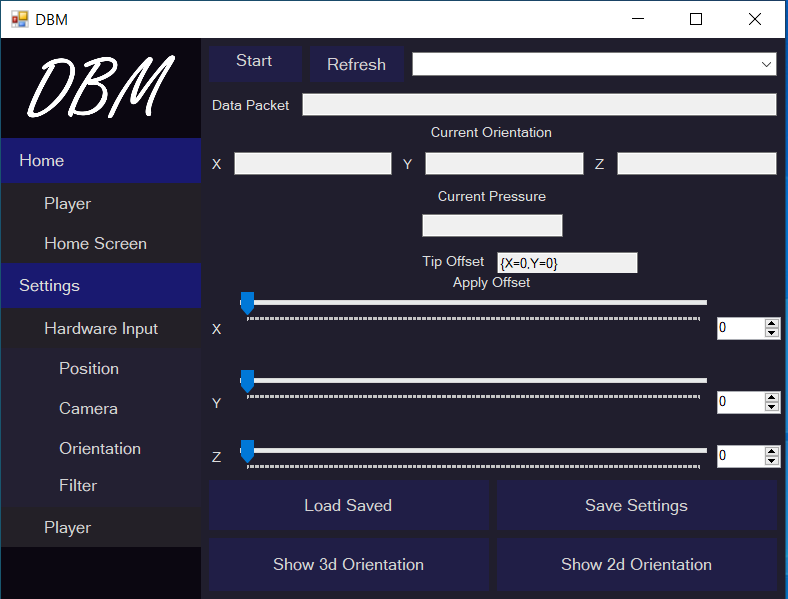
\includegraphics[width=12cm, height=11cm]{Controller App Orientation Calibration}
  \caption{Controller App Orientation Calibration}
\end{figure}

\subsection{3d Orientation Screen}
When ‘Show 3d Orientation’ button from Orientation Calibration Form is clicked, 3d Orientation form is displayed. It shows orientation of marker in three-dimensional space. Box of 3d model show tail of the marker and conical head show tip of marker.

\newpage
\begin{figure}[h]
  \centering
  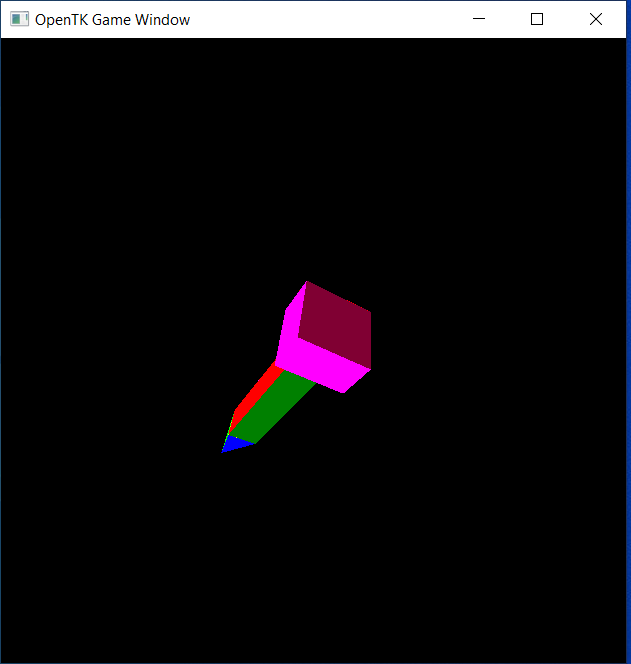
\includegraphics[width=10cm, height=8cm]{Controller App Orientation Visualization}
  \caption{Controller App Orientation Visualization in 3d Space}
\end{figure}

\subsection{2d Orientation Screen}
When ‘Show 2d Orientation’ button from Orientation Calibration Form is clicked, 3d Orientation form is displayed. It shows orientation of marker in three-dimensional space. Box of 3d model show tail of the marker and conical head show tip of marker.
\begin{figure}[h]
  \centering
  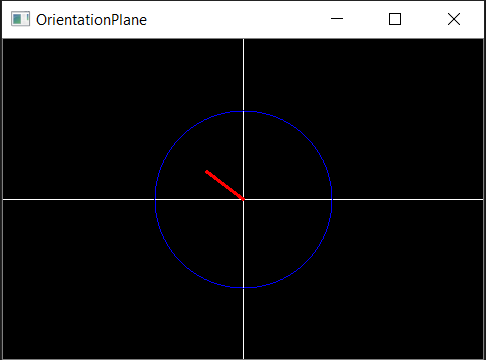
\includegraphics[width=10cm, height=8cm]{Controller App 2d Orientation Visualization}
  \caption{Controller App Orientation Visualization in 2d Space}
\end{figure}

\subsection{Filter Control Panel Screen}
When Settings->Hardware Input->Filter from navigation bar is clicked, Filter Control Panel form is displayed. Role of this form is to perform computer vision algorithms and filters to get the position of the glowing ball of the board marker. It contains at least two sub-forms that contain settings of each camera filter. Each filter form contains the following controls:

\begin{enumerate}

\item Upper Limit group-box: Contains three trackbars that is used to adjust the upper limit of color filter in HSV color space.
\item Lower Limit group-box: Contains three trackbars that is used to adjust the lower limit of color filter in HSV color space.
\item Preview button: Launches the filter preview form.
\item Load Saved button: Load saved settings from the local storage.
\item Save Settings button: Save the settings on local storage.

\end{enumerate}


\begin{figure}[h]
  \centering
  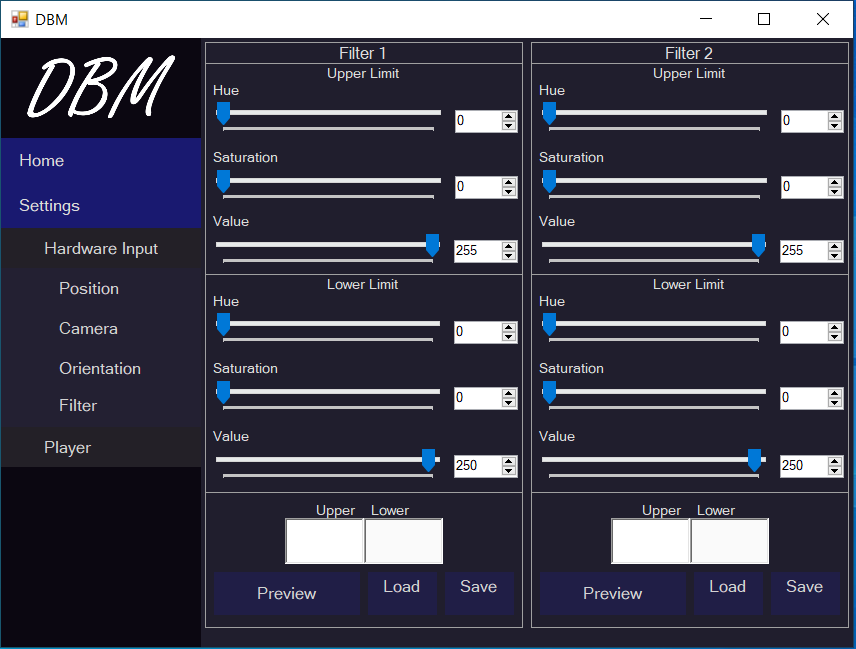
\includegraphics[width=12cm, height=11cm]{Controller App Filter Control Panel}
  \caption{Controller App Camera Filter Control Panel}
\end{figure}

\subsection{Filter Preview Screen}
When ‘Preview’ button from Filter Control Panel Form is clicked, 3d Orientation form is displayed. Role of this form is to display the mask applied to camera to extract the position of glowing ball. It contains the following controls:

\begin{enumerate}

\item Offset textbox: Displays the relative position of glowing ball with respect to mid. It displays the value in percentage.
\item Show Mask: Toggle show filter and normal preview.
\item Undo button: undo last placed dot on this preview screen.
\item Preview Screen: Dots i.e. particularly three, can be placed. First two dots display a line that is aligned with the surface of Board. Third dot display the corner of the board just ahead of the camera.
\item Load Saved button: Load saved settings from the local storage.
\item Save Settings button: Save the settings on local storage.

\end{enumerate}

\begin{figure}[h]
  \centering
  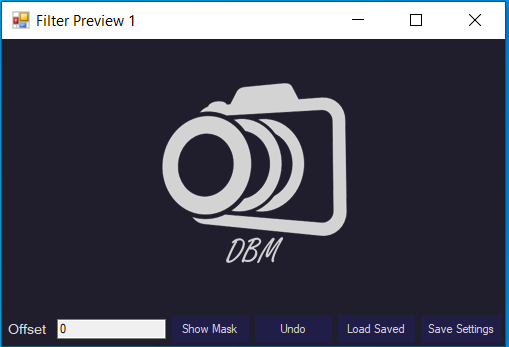
\includegraphics[width=12cm, height=11cm]{Controller App Filter Preview}
  \caption{Controller App Camera Filter Preview}
\end{figure}

\subsection{Flow Diagram}
The general flow diagram of controller application is given below:

\begin{figure}[h]
  \centering
  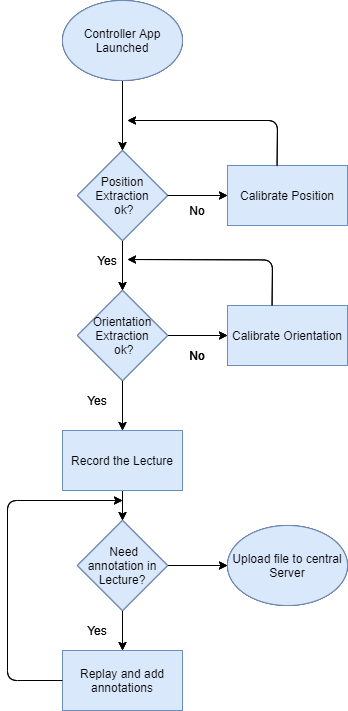
\includegraphics[width=8cm, height=10cm]{Controller App}
  \caption{Controller App Flow Diagram}
\end{figure}

\subsection{Rules and Assumptions}
Following are rules and cases of assumptions that are assumed to be true while normal working:

\begin{itemize}

\item Application is not closed while recording otherwise all recording will be wasted.

\end{itemize}

\subsection{Tools and Technologies used}
List all software that are used to develop and needed to operate the developed module are detailed below:

\subsection{Visual Studio 2019}
Code environment in which all code for Controller application is written. This IDE is numerously used as a debugging tool as well.

\textbf{Libraries Used}\mbox{}\\
Following external libraries are used while development of controller application:

\begin{itemize}

\item Newtonsoft.Json v12.0.3: To serialize and deserialize data into and from Json objects.
\item ColorMine v1.1.3: For Inter-conversion of color spaces i.e. RGB and HSV
\item EMGU.CV v4.1.1.3497: OpenCV image processing library used in capturing and filter formation.
\item DirectShowLib v1.0.0: Used to get list of all connected cameras.
\item OpenTK v3.1.0: Used to render 3d model of marker for orientation calibration.

\end{itemize}

\section{Player Application}
This module acts just like regular media player that play video file. The difference is that it plays a lecture file only, generated by controller application. File if of .dbm extension.\\
Player application has navigation bar on left side that control panel and sub-panels that contain buttons. Buttons navigate to the corresponding form. A hierarchy that describe the categorization of forms is given below:

\begin{enumerate}

\item Home Panel
\begin{enumerate}[a.]

\item Player
\item Home Screen

\end{enumerate}


\item Settings Panel
\begin{enumerate}[a.]

\item Player Settings

\end{enumerate}

\end{enumerate}

Complete description along with UI screens of controller application are given below

\subsection{Player Screen}
When ‘Player’ button from navigation bar is clicked, Player screen is displayed. It contains the following controls

\begin{enumerate}

\item Seek bar: Indicates the current playing time of the lecture video. It also indicates how much video as passed and how much is remaining.
\item Start Playing button: Plays the recorded lecture.
\item Load File button: To load the recorded lecture file. It will open a file browser from which a file with .dbm extension is selected.
\item Thickness Trackbar: Controls the line thickness of writing being written and also duster size.
\item Load Saved button: Load the saved settings on local storage.
\item Save Settings button: Save the settings from local storage.
\item Canvas: Black window on which words are being written i.e. Board.

\end{enumerate}

\begin{figure}[h]
  \centering
  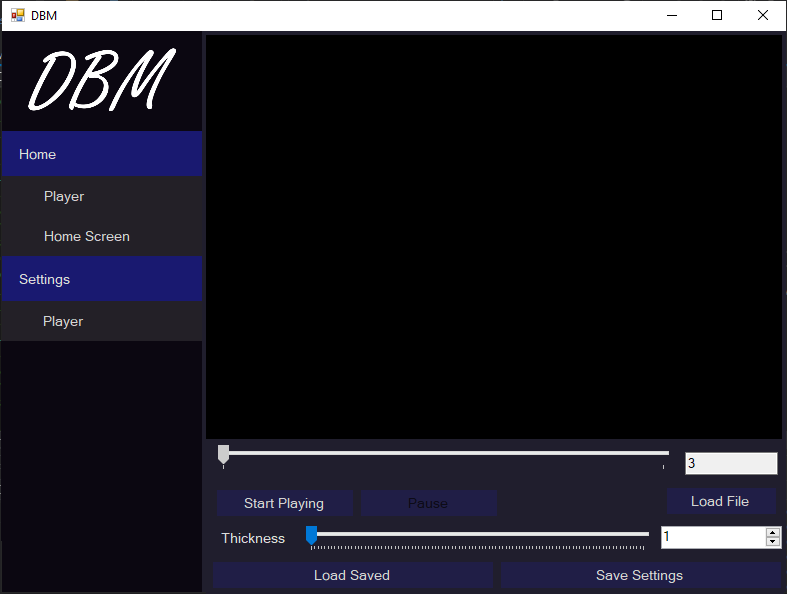
\includegraphics[width=13cm, height=13cm]{Player App (2)}
  \caption{Player Application Main Screen}
\end{figure}

\newpage
\subsection{Flow Diagram}
\begin{figure}[h]
  \centering
  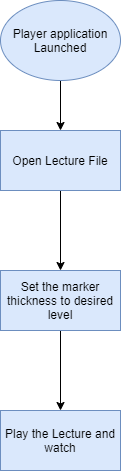
\includegraphics[width=5cm, height=10cm]{Player Application}
  \caption{Player App Flow Diagram}
\end{figure}

\subsection{Tools and Technologies used}
List all software that are used to develop and needed to operate the developed module are detailed below.

\subsubsection{Visual Studio 2019}
Code environment in which all code for Controller application is written. This IDE is numerously used as a debugging tool as well.

\textbf{Libraries Used}\\
Following external libraries are used while development of controller application:

\begin{itemize}

\item Newtonsoft.Json v12.0.3: To serialize and deserialize data into and from Json objects.
\item ColorMine v1.1.3: For Inter-conversion of color spaces i.e. RGB and HSV
\item EMGU.CV v4.1.1.3497: OpenCV image processing library used in capturing and filter formation.

\end{itemize}












































